%!TEX root = main.tex

\section{Data}
\label{sec:dataset}

We begin this section with the description of our packet-level data from a mobile voice search service, and then provide high-level statistics of TCP performance. 

\subsection{Data Collection}

\begin{figure}[th]
	\centering
	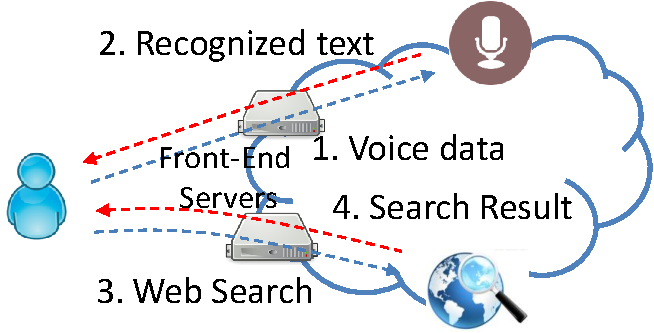
\includegraphics[width=0.8\linewidth]{voice_search_process}
	\caption{Voice search engine infrastructure.}
	\label{fig:voice_search}
\end{figure}

We collect mobile voice search data from one of the top 3 search service providers in China. This service provider serves more than 400 million users per day. A voice search initialized from a mobile terminal consists of two successive phases as shown in Figure~\ref{fig:voice_search}: \emph{voice recognition} (\ie recognize speech to query text) and \emph{web search} (\ie search with returned query text). Voice recognition and web search are served by different servers through HTTP. As such, a voice search session consists of two separate TCP flows.

We collect packet-level traces from front-end servers\footnote{Note that our traces are from a subset (3) of all servers, and given the load-balancing done across these, our data likely represents a uniform random flow sample.} of both voice recognition and web search, resulting in two datasets that correspond to the two phases of voice search. The front-end servers from which we obtained the data provide services for mobile users in the same geographical locations. As the service provider relies on geographically-biased server selection, we assume that the flows in the two datasets cross networks with similar characteristics. The web search servers provide search services for both voice search and traditional user-type search. The datasets were collected in April 2015 for two weeks. In total, we obtained about 1 million voice recognition flows and 3 million web search flows.

%We report measurement results for each of the two phases of voice search.

All voice search requests are originated from mobile apps, especially from the Android platform, either via cellular or WiFi access network. About 2.5\% of the voice recognition flows and 6.7\% of the web search flows originate from the cellular network, made of a mixture of technologies: 2.5G, 3G and 4G\footnote{The cellular network type was inferred using the HTTP header field ``x-up-bear-type''.}. However, we observed a very limited number of 2.5G and 4G flows (less than 0.5\% of the total flows) in our data\footnote{Indeed, 4G is still in its initial stages of deployment in China and has limited coverage.} and thus omit them from our analysis. In total, they make up about 2.5\% of the flows.

\begin{figure}[th]
\centering
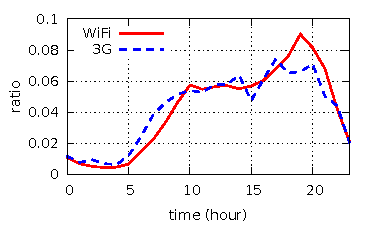
\includegraphics[width=0.8\linewidth]{voice_time_rate}
\caption{Distribution of voice search requests in a day.}
\label{fig:voice_time_rate}
\end{figure}

Figure~\ref{fig:voice_time_rate} shows the distribution of voice search flows over time of a day. Flows are binned into 1-hour frame and we report the ratio of flows in each interval divided by the daily total. Not surprisingly, we observe a sharp increase of the search volume from 5AM to 10AM. The search volume from 3G remains relatively stable over the day and declines around 10PM, while we observe continuous growth of the WiFi search which reaches its peak at 7PM. The daily trend for web search flows is similar (not show). The daily search volume variation trend we observe is very similar to the one previously reported by \cite{Song:2013:EEU:2488388.2488493} for Bing mobile search.

\subsection{TCP Performance Measures}

\begin{figure}[ht]
\centering
\begin{subfigure}[b]{0.6\linewidth}
	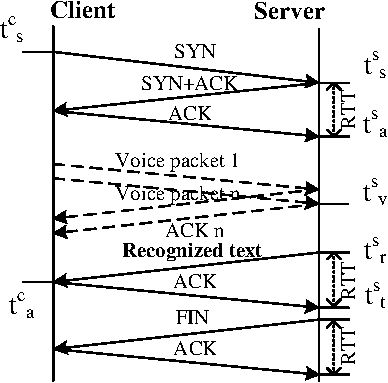
\includegraphics[width=\textwidth]{voice_estimate_rtt}
\caption{Voice recognition}
\label{fig:voice_estimate_rtt}
\end{subfigure} \\
%\vspace{0.1in}
\begin{subfigure}[b]{0.6\linewidth}
	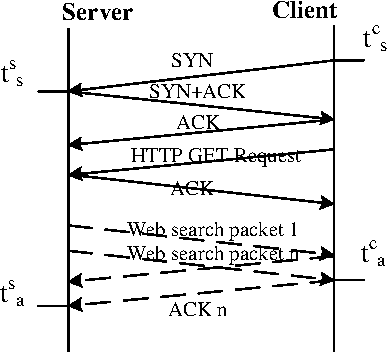
\includegraphics[width=\textwidth]{web_finish_time_example}
\caption{Web search}
\label{fig:web_finish_time_example}
\end{subfigure}
\caption{Time-line of a voice recognition flow and a web search flow.}
\label{fig:time_line}
\end{figure}

% For a voice search session, both the voice recognition and the web search phases contribute to the performance. However, they could have very distinct behavior as seen from the server-side. This is because as shown in Figure \ref{fig:time_line}, in the voice recognition phase, the server acts as a TCP receiver, while in the web search phase, the server is the sender. Note that TCP is largely a sender-driven transmission protocol and its transmission performance is affected by the ability of the sender to handle congestion events, as well as the ability of the receiver to receive data. We examine the TCP performance factors of each phase for individual voice search sessions and their impact on the flow \emph{flow completion time}.

User perceived response time of a mobile voice search session is affected by the \emph{completion time} of the voice recognition flow as well as that of the web search flow. Here, the completion time of a flow measures the duration from the time when client initiates the connection till the time when the last byte of data is acknowledged. We define the completion time for the flows in the two phases separately as follows.

Voice recognition consists of mobile terminals uploading the voice data and server returning back the recognized query text as shown in Figure~\ref{fig:voice_estimate_rtt}. The following web search is initialized by mobile clients once they receive the recognized text (encapsulated in one packet) at $t^c_a$. That said, the completion time of a recognition flow measures the duration from $t^c_s$ to $t^c_a$. Unfortunately, we do not have these two timestamps at server side where we collected our datasets. Note that the timestamp option in TCP is disabled since otherwise, clients behind NATs (Network Address Translations) might not be able to build connections with the servers that with PAWS (Protect Against Wrapped Sequence number) \cite{rfc7323} enabled \cite{Wang:2011:USM:2018436.2018479}. Alternatively, we approximate the flow completion time with $T_s=t^s_t - t^s_s$. This flow completion time however includes the time consumed by servers to translate speech to text ($T_r=t^s_r - t^s_v$), which is not relevant to network performance\footnote{The time duration needed for translating voice to text is dependent on the used speech recognition technology. We refer interested readers to \cite{36463,schalkwyk2010your} for more details regarding speech recognition.} and therefore out of scope in this paper. We thus redefine the flow completion time of a voice recognition flow as $T_s-T_r$.

Web search starts when a mobile terminal initiates a connection to transmit the query text, and ends when the server receives ACKs for all returned search results as shown in Figure~\ref{fig:web_finish_time_example}. Note that for the web search phase, we only consider flows carrying search results that are dynamically generated by servers based on the query and ignore those corresponding to static content such as CSS/JavaScript files. This is because the performance for static content (as opposed to the dynamic search results) can be optimized easily through CDN (Content Delivery Network) caching. The flow completion time at the client-side is the duration between transmitting the SYN packet $t^c_s$ and receiving all web search data $t^c_a$. We use the duration $T_s=t^s_a - t^s_s$ measured at the server-side to approximate the latency that the user perceives. Again, we excluded the time consumed by servers processing the query $T_r=t^s_r - t^s_q$ and obtained the flow completion time as $T_s-T_r$.

\begin{figure}[t]
\centering
\begin{subfigure}[b]{0.8\linewidth}
	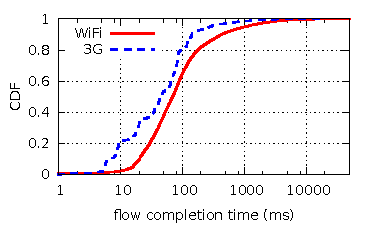
\includegraphics[width=\textwidth]{voice_finish_time}
\caption{Voice recognition}
\label{fig:voice_finish_time}
\end{subfigure} \\
%\vspace{0.1in}
\begin{subfigure}[b]{0.8\linewidth}
	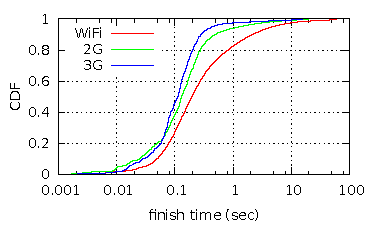
\includegraphics[width=\textwidth]{web_finish_time}
\caption{Web search}
\label{fig:web_finish_time}
\end{subfigure}
\caption{CDFs of flow completion time in the two phases.}
\label{fig:finish_time}
\end{figure}


Figure~\ref{fig:finish_time} plots the cumulative distribution (CDF) of the flow completion time of TCP flows in the two phases, where $x$-axis is in log scale. Interestingly, we find that in both phases 3G flows experience a shorter completion time than WiFi flows. Furthermore, some flows experience a very large completion time compared to others, displaying a heavy tailed behavior that was also found in Google search \cite{flach2013reducing}. For example, while most of the voice recognition flows finish in 100ms, a non-negligible fraction of flows (5\% in WiFi, and 2\% in 3G) take more than 1 second to upload the voice data. 

%Figure~\ref{fig:web_finish_time} shows the CDF of flow completion time of web search flows. In the figure, the overall completion time of flows in 2G and 3G (with median values 0.013s and 0.011s) in also shorter than that of flows in WiFi network (with median value 0.2s). More than 25\% of flows in all networks experience completion time less than 0.1 second. However, 5\% of flows in 2G network and 18\% in WiFi network experience completion time more than 1 second. Furthermore, about 3\% of flows in WiFi network are with completion time more than 10 seconds, which is a great performance degradation.

A comparison of the TCP flow completion time between voice recognition and web search in Figure~\ref{fig:finish_time} shows that the flow completion time in web search contributes to the majority of the user-perceived (network-related) performance of a voice search session. However, it does not mean that understanding the performance of voice recognition flows is not as important as for web search flows. Indeed, voice recognition is the first step of the whole voice search process, and therefore a long recognition time would certainly result in bad user experience, potentially even early termination of the process.

% These observations motivate our analysis of the TCP performance and its impact on the flow completion time in each phase of the mobile voice search.

% some of voice recognition flows suffer from timeout retransmission, which is a great performance degradation~\cite{flach2013reducing}. Second, a non-negligible fraction of voice recognition flows are terminated before voice data transmission completes. These bad user experiences also inspire us to understand what factors and how they impact user-perceived performance in voice recognition flows.

We were motivated by the above observations to have an in-depth analysis of the TCP performance in mobile voice search. To this end, we focus on the following three most important aspects of TCP performance.

\begin{itemize}
	\item {Round Trip Time (RTT):} RTT is a commonly used indicator of TCP performance, especially for short TCP flows like search flows.
	
	\item {Number of lost/disordered packets:} Both packet loss and packet reordering could affect the transmission time. Packet loss leads to a reduction of the sender congestion window. Although packet reordering does not reduce the congestion window, it can prevent the congestion window from growing and may trigger spurious retransmissions.
	
	\item {Timeout Retransmission:} In timeout retransmission, the TCP sender has to wait for a RTO (Retransmission Timeout) before retransmitting the lost packet. The RTO can be tens of RTTs. Such kind of ``expensive'' retransmissions can degrade TCP performance, especially for short flows like those considered in this paper~\cite{flach2013reducing}.

\end{itemize}

%When examining the impact of the above factors on TCP flow completion time, we also consider the potential impact of TCP flow size. We are particularly interested in the disparity that might exist when issuing voice searches from 3G and WiFi. 
TCP is a sender-driven transmission protocol and its performance is mainly affected by the sender-side factors. However, as shown in Figure \ref{fig:time_line}, the server acts as a TCP receiver in the voice recognition phase. As such, we cannot obtain the statistics of the above TCP performance factors of the sender in the voice recognition phase. Alternatively, we infer as much information as we can for these factors. The server in the web search phase is on the other hand the TCP sender, and thus we can have a better view of how the TCP sender behavior and its impact on the flow completion time. In addition, we are particular interested in the disparity that might exist when issuing voice searches from 3G and WiFi. 
